\chapter{Nasazení}
\label{sec:dp}

\begin{figure}[h!]
    \centering
    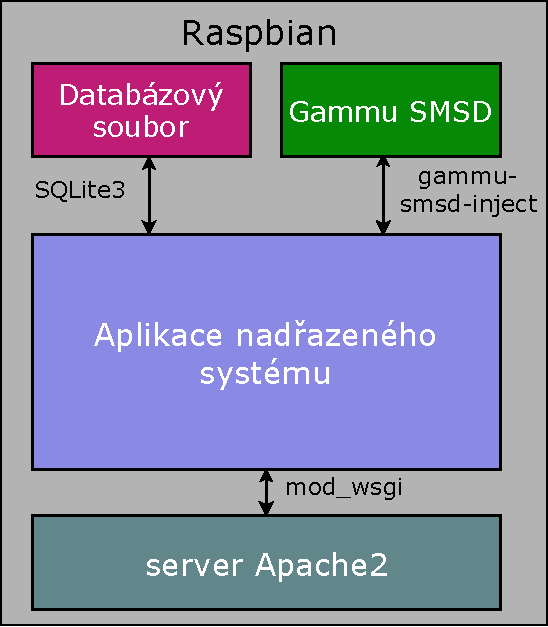
\includegraphics[width=0.8\textwidth]{images/sw_block.pdf}
    \caption[Softwarové blokové schéma nadřazeného systému]{Softwarové blokové schéma nadřazeného systému. Aplikace běží na OS Raspbian. Jako webový server je použit Apache2, se kterým aplikace komunikuje pomocí modulu mod\_wsgi \cite{mod_wsgi}. Databáze je upravována pomocí systému SQLite3, pro odesílání SMS s upozorněními je použit program Gammu (bližší informace v sekci \ref{sec:im_notifications}).}
    \label{fig:sw_block}
\end{figure}

V této kapitole je stručně popsáno nasazení aplikace nadřazeného systému na jednodeskovém počítači Raspberry Pi 3 s operačním systémem Raspbian. Blokové schéma nasazené aplikace je na obrázku \ref{fig:sw_block}. 

K instalaci a spuštění aplikace je zapotřebí tento software:

\begin{itemize}
    \item Webový server Apache2.
    \begin{itemize}
        \item Nutno nainstalovat modul mod\_wsgi  \cite{mod_wsgi}.
    \end{itemize}
    \item Programovací jazyk Python3.
    \begin{itemize}
        \item Systém pro správu balíčků pip. Díky němu lze snado nainstalovat všechny potřebné Python moduly, jako například Flask nebo SQLAlchemy.
    \end{itemize}
    \item Program pro ovádání GSM modulu Gammu. Nadřazený systém je možné spustit i bez instalace tohoto programu, pouze nebude fungovat zasílání SMS upozornění.
\end{itemize}

\newpage

\section{Konfigurace Apache2}

Po instalaci potřebného softwaru je nejprve nutné nakonfigurovat server Apache2, aby doručoval aplikaci nadřazeného systému. 

K doručení Python aplikace je použit modul mod\_wsgi, jehož základní konfigurace je popsána v článku \cite{flask_wsgi}. Spuštění aplikace pomocí mod\_wsgi je provedeno pomocí skriptu z ukázky \ref{lst:wsgi_script}.

\begin{listing}[htbp]
\caption{\label{lst:wsgi_script} Skript pro spuštění aplikace na serveru Apache2 pomocí modulu mod\_wsgi. Tento skript importuje objekt aplikace nadřazeného systému (\texttt{app}), který je pak používán WSGI modulem \cite{flask_wsgi}.}
\inputminted[bgcolor=codebg]{python}{source-samples/wsgi.py}
\end{listing}

\newpage

\subsection{Přístup k databázi a \texttt{user\_config.ini}}

Aplikace nadřazeného systému potřebuje měnit obsah databáze a souboru s uživatelským nastavením. Je tedy nutné povolit uživateli, pod kterým aplikace běží, čtení a zápis těchto souborů. 

Apache2 spouští aplikace jako uživatel \texttt{www-data}, přístup k souborům je tedy možné povolit způsobem popsaným v ukázce \ref{lst:wwwdata}.

\begin{listing}[htbp]
\caption{\label{lst:wwwdata} Nastavení přistupových práv k databázi a souboru s uživatelským nastavením.}
\inputminted[bgcolor=codebg]{bash}{source-samples/wwwdata.sh}
\end{listing}


\subsection{Konfigurace HTTPS}

% zapnout mod_ssl

\section{Konfigurace Gammu SMSD}

\section{Konfigurace RTC}